\documentclass{article}
\usepackage[utf8]{inputenc}
\usepackage{amssymb}
\usepackage{tikz}
\usepackage{tikz-cd}

\title{LogMathsHW3}
\author{Louis-Hendrik Barboutie}
\date{April 2022}

\begin{document}

\maketitle

\section{First Part}


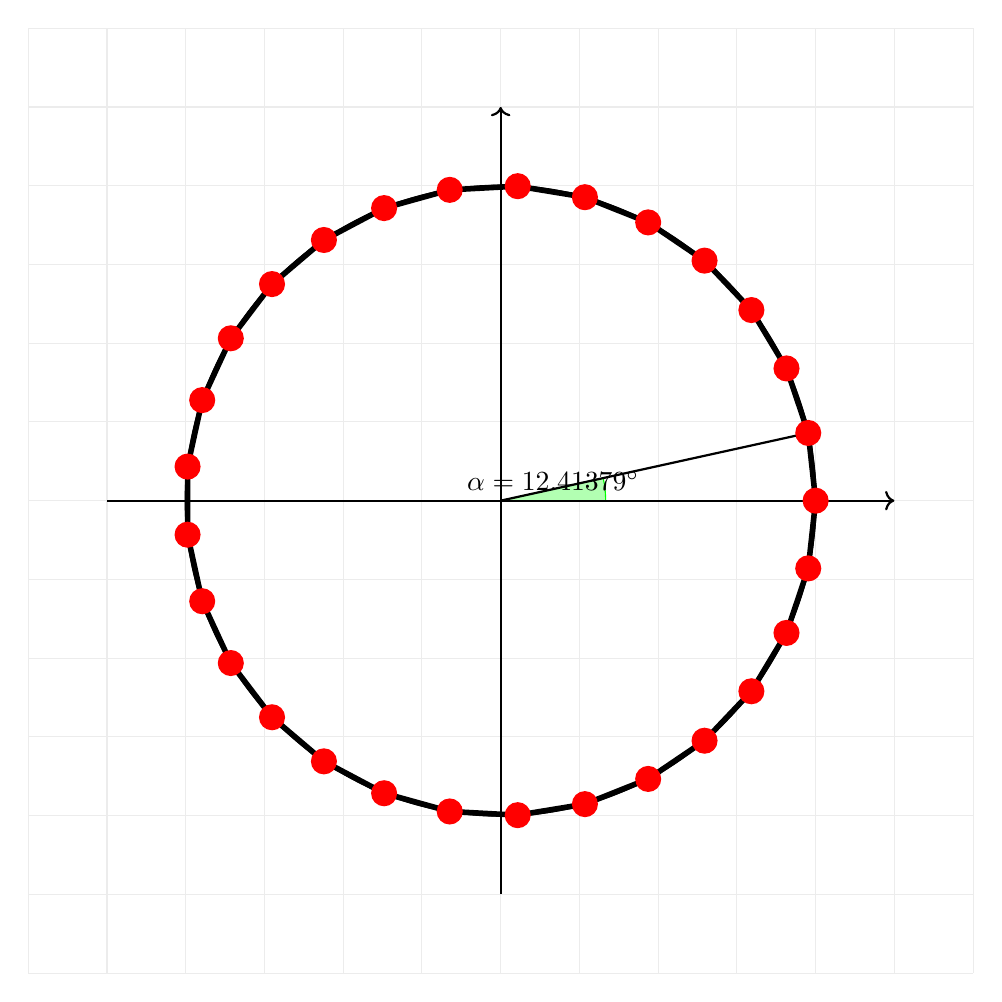
\begin{tikzpicture}
\tikzset{anglefill/.style={draw=green,fill=green!30}}
\pgfmathsetmacro{\N}{29}
\pgfmathsetmacro{\r}{4}
\pgfmathsetmacro{\a}{360/\N}
\draw[lightgray!30] (-6,-6) grid[step=1] (6,6);
\filldraw[anglefill] (0,0) -- node[above]{$\alpha = \a^\circ$}
(\r/3,0) arc [start angle=0,end angle= {360/\N},radius=\r/3] -- cycle;
\draw[thick,->] (-5,0) -- (5,0);
\draw[thick,->] (0,-5) -- (0,5);
\draw[thick] (0,0) circle[radius=\r] -- ({360/\N}:\r);
\foreach \i in {1,...,\N}
{
    \draw[line width = 2pt] ({360/\N * (\i -1)}:\r) -- ({360/\N * (\i )}:\r);
}
\foreach \i in {1,...,\N}
{
    \node[fill, circle=20pt,red] at ({360/\N * (\i -1)}:\r) {};
}
\end{tikzpicture}


\section{Second Part}

\begin{center}
    \begin{tikzcd}
        0 \arrow[r] & A' \arrow[d] \arrow[r, hookrightarrow] & A \arrow[d, "\sim"] \arrow[r, twoheadrightarrow] & A'' \arrow[d] \arrow[l, dashed, bend right, "s"'] \arrow[r] & 0 \\ 
        0 \arrow[r] & A' \arrow[r, hookrightarrow, "i_{A'}"'] & A' \oplus A'' \arrow[r, twoheadrightarrow, "\pi_ {A''}"'] & A'' \arrow[r] & 0
    \end{tikzcd}
\end{center}

\end{document}
